\problemname{Battleship}

In this exercise, you will program a computer game:
\href{https://en.wikipedia.org/wiki/Battleship_(game)}{Battleship!}
For the sake of simplicity, we will limit ourselves to a single-player mode with one board.
At the start of the game, $5$ ships are placed on a grid with $10 \times 10$ tiles.

The grid's columns are numbered from $1$ to $10$
whereas the rows are labelled using the letters \texttt{A} to \texttt{J} (see image below).
Individual coordinates are referenced by letter and number, e.g. \texttt{D9} or \texttt{J10}.

\begin{figure}[h]
    \centering
    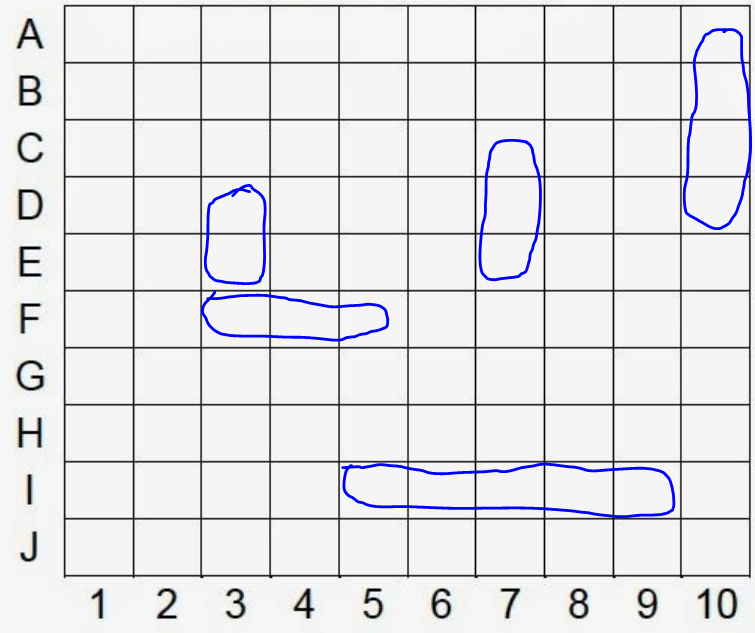
\includegraphics[width=0.33\textwidth]{battleship-grid}
    \caption{\texttt{Battleship grid}}
\end{figure}
The ships are placed either horizontally or vertically on the grid.
The ships sizes are as follows:
\begin{itemize}
    \item The carrier is the biggest and occupies $5$ tiles.
    \item The battleship occupies $4$ tiles.
    \item The destroyer and submarine, both occupy $3$ tiles.
    \item Finally, the patrol boat that occupies $2$ tiles.
\end{itemize}

\section*{Input}
The input starts with the program prompting the user for the location of each of the five ships with\\
``\texttt{Location and orientation of your \{ship type\}:\textbackslash n}''.\\
The second part of the input then consists of $n$ lines, 
where each line $n_i$ contains one attack.

In the tests, $n$ will be restricted to $17 \le n \le 100$.
It is also guaranteed that the placements of all ships will be valid, 
that is to say no ship overlaps another.

In the samples below,
the first five lines contain the placement of the ships.
The remaining $n$ lines each contain one attack made by the player.

\section*{Output}
The output should start with $n$ lines, one for each attack the player made,
where the program outputs one of the following:
\begin{itemize}
    \item ``\texttt{Miss.}'' if the attack missed.
    \item ``\texttt{Hit, \{ship type\}.}'' if the attack hit a ship.
    \item ``\texttt{You have sunk my \{ship type\}.}'' if all of the ship's tiles have now been attacked.
\end{itemize}
Then finally when all the ships have been sunk, the program should print ``\texttt{The entire fleet has been sunk.}'' and exit.
